% =====================================================================
%  Guía de la plantilla — EJEMPLOS DE USO. BORRAR antes de entregar
%  (quitar la línea \include{anexos/anexo_guia_plantilla} en main.tex).
%  Sirve de referencia rápida para ti y para cualquier IA.
%  Formato de títulos, leyendas y citas según 01_normativa/REGLAS_FORMATO.md.
% =====================================================================
\chapter{Guía rápida de la plantilla (borrar)}
\label{anx:guia}

\section{Ecuaciones}
\label{sec:guia-ecuaciones}

La ecuación de Manning para flujo uniforme en canales abiertos es:
\begin{equation}
  V = \frac{1}{n} R_h^{2/3} S^{1/2}
  \label{ec:manning}
\end{equation}
donde $V$ es la velocidad media (\unit{\meter\per\second}), $n$ el coeficiente de rugosidad, $R_h$ el radio hidráulico (\unit{\meter}) y $S$ la pendiente.
La \cref{ec:manning} está en unidades del SI\@.

Ecuaciones alineadas, por ejemplo la ecuación de movimiento de un sistema de un grado de libertad~\parencite{suarez2014analisis}:
\begin{align}
  m\ddot{u} + c\dot{u} + k u &= -m\ddot{u}_g(t) \label{ec:eom}\\
  \omega_n &= \sqrt{k/m}
\end{align}

\section{Unidades con siunitx}

Hormigón de $\fc = \qty{25}{\mega\pascal}$, carga de \qty{12.5}{\kilo\newton\per\meter}, rango de \qtyrange{2}{4}{\meter}, peso de \qty{3.2}{\tonf}.
Los números se formatean solos: \num{1234567.89}.

\section{Figuras}

\subsection{Figura generada por Python}

La \cref{fig:ejemplo-python} se genera con \texttt{04\_analisis/scripts/ejemplo\_figura.py}; si cambian los datos, se vuelve a correr y la tesis se actualiza.
\begin{figure}[htbp]
  \centering
  \includegraphics[width=0.7\textwidth]{ejemplo_vibracion.pdf}
  \caption{Vibración libre amortiguada de un oscilador de un grado de libertad (figura de ejemplo).}
  \label{fig:ejemplo-python}
\end{figure}

\subsection{Diagrama con TikZ}

Toda figura se menciona en el texto \emph{antes} de que aparezca, como la \cref{fig:tikz-flujo}.

\begin{figure}[htbp]
  \centering
  \begin{tikzpicture}[
      caja/.style={rectangle, draw, rounded corners, minimum width=3cm, minimum height=0.9cm, align=center, fill=blue!5},
      flecha/.style={-{Stealth}, thick}]
    \node[caja] (a) {Revisión\\bibliográfica};
    \node[caja, right=1cm of a] (b) {Modelación};
    \node[caja, right=1cm of b] (c) {Análisis de\\resultados};
    \node[caja, below=1cm of b] (d) {Validación};
    \draw[flecha] (a) -- (b);
    \draw[flecha] (b) -- (c);
    \draw[flecha] (b) -- (d);
    \draw[flecha] (d) -| (c);
  \end{tikzpicture}
  \caption{Diagrama de flujo de metodología dibujado con TikZ. Fuente: elaboración propia.}
  \label{fig:tikz-flujo}
\end{figure}

\subsection{Esquema estructural con TikZ}

La \cref{fig:viga} muestra un esquema dibujado con código.

\begin{figure}[htbp]
  \centering
  \begin{tikzpicture}[scale=1.2]
    % viga
    \draw[very thick] (0,0) -- (6,0);
    % apoyos
    \draw (0,0) -- (-0.25,-0.4) -- (0.25,-0.4) -- cycle;
    \draw (6,0) -- (5.75,-0.4) -- (6.25,-0.4) -- cycle;
    \draw (5.7,-0.5) -- (6.3,-0.5);
    % carga distribuida
    \foreach \x in {0,0.5,...,6} \draw[-{Stealth}] (\x,0.8) -- (\x,0.05);
    \draw (0,0.8) -- (6,0.8);
    \node[above] at (3,0.8) {$q = \qty{10}{\kilo\newton\per\meter}$};
    % cota
    \draw[{Stealth}-{Stealth}] (0,-0.8) -- node[below] {$L = \qty{6}{\meter}$} (6,-0.8);
  \end{tikzpicture}
  \caption{Viga simplemente apoyada con carga uniforme.}
  \label{fig:viga}
\end{figure}

\subsection{Gráfico con PGFPlots}

La \cref{fig:momento} es un gráfico calculado por LaTeX.

\begin{figure}[htbp]
  \centering
  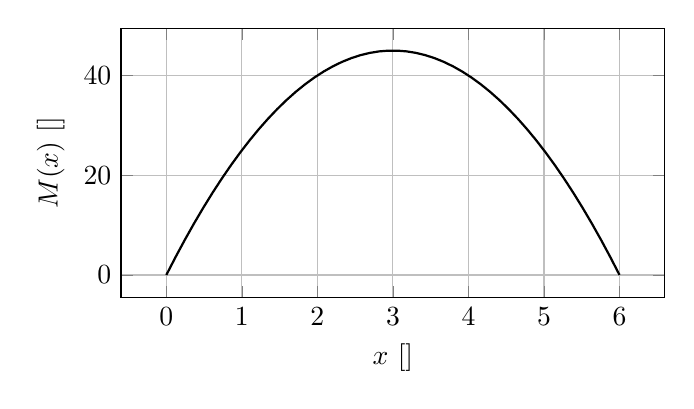
\begin{tikzpicture}
    \begin{axis}[width=0.7\textwidth, height=5cm, xlabel={$x$ [\unit{\meter}]}, ylabel={$M(x)$ [\unit{\kilo\newton\meter}]}, grid=major]
      \addplot[thick, domain=0:6, samples=50] {10*x/2*(6-x)};
    \end{axis}
  \end{tikzpicture}
  \caption{Momento flector de la viga de la \cref{fig:viga}: $M(x) = \tfrac{q x}{2}(L-x)$.}
  \label{fig:momento}
\end{figure}

\section{Tablas}

La \cref{tab:ejemplo} viene de un archivo generado por Python, guardado en \texttt{tablas/}.
\begin{table}[htbp]
  \centering
  \caption{Tabla generada automáticamente desde \texttt{04\_analisis}.}
  \label{tab:ejemplo}
  \input{tablas/ejemplo_tabla}
\end{table}

\section{Citas (APA 7)}

Los ejemplos oficiales de los Lineamientos, en APA~7:
libro~\parencite{suarez2014analisis},
artículo científico~\parencite{zhou2026performance},
norma~\parencite{inn2009nch433}
y sitio web~\parencite{mop2026proyectos}.
Cita narrativa: \textcite{zhou2026performance} proponen\dots
Si falta una fuente: \pendiente{falta fuente para el valor del coeficiente}.
Si algo es dudoso: \revisar{¿este valor corresponde a la norma vigente?}
